\subsection{Teoria Sterowania}

Teoria sterowania (ang. \textit{control theory}) jest to dziedzina inżynierii oraz matematyki stosowanej, która mierzy się z kontrolowaniem układów dynamicznych \footnote{\url{https://en.wikipedia.org/wiki/Dynamical_system}} w procesach inżynieryjnych i maszynach. Jej celem w danym problemie jest opracowanie modelu lub algorytmu, który zarządza sygnałami wejściowymi do systemu tak, aby osiągnął on stan docelowy. 

W tym celu potrzebny jest regulator (ang. \textit{control system}). Regulator zarządza, steruje, kieruje lub reguluje zachowanie innych urządzeń lub systemów, wykorzystując pętle sterowania. Regulator monitoruje kontrolowaną zmienną procesu (ang. \textit{process variable}) (PV) i porównuję ją z wartością odniesienia (ang. \textit{set point}) (SP). Różnica między rzeczywistą a pożądaną wartością zmiennej procesu, nazywana sygnałem błędu lub uchybem regulacji jest stosowana jako sprzężenie zwrotne w celu wygenerowania sygnału sterującego, które doprowadzi kontrolowaną zmienną procesu (PV) do wartości równej punktowi odniesienia (SP).

\subsubsection{Układ automatycznej regulacji}
\begin{figure}[!h]
    \centering 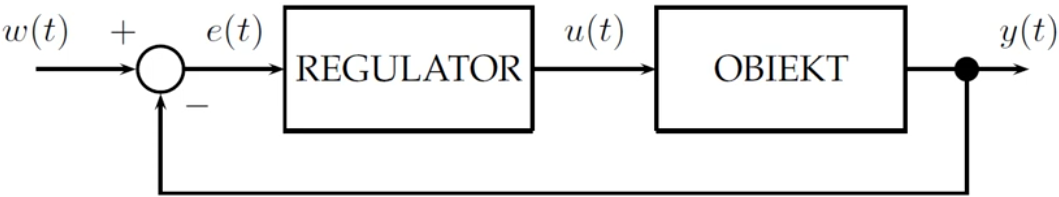
\includegraphics[width=1\linewidth]{25-uar.png}
    \caption{Układ automatycznej regulacji (UAR)}\label{fig:25-uar}
\end{figure}

Jeśli chcemy kontrolować wyjście danego obiektu zamykamy układ sprzężeniem zwrotnym. Wykonujemy pomiaru sygnał wyjściowego $y(t)$  i porównujemy z sygnałem odniesienia $w(t)$ (\textit{ang. set point}). Otrzymujemy w ten sposób \textit{uchyb regulacji} $e(t)$, który trafia do regulatora. Regulator przetwarza dostarczony mu uchyb i na tej podstawie wytwarza sygnał sterujący zarządzanym obiektem, czyli sygnał $u(t)$ zwany również wymuszeniem.

Przykładem może być układ regulacji temperatury obiektu, gdzie regulator ma postać przekaźnika dwupołożeniowego (Rys. \ref{fig:25-termostat}). Jeżeli jest za zimno załącza się stan wysoki, czyli ogrzewanie. Jeżeli jest za gorąco włącza się stan niski czyli chłodzenie. Punktem odniesienia $w(t)$ jest tutaj temperatura 21 stopni. Gdy \textit{pomiar} $y(t)$ znajduje się poniżej tej wartości, obliczany \textit{uchyb regulacji} $e(t)$ przyjmuje wartość dodatnią. Regulator jest zaprogramowany w taki sposób (wykonuje taki algorytm), że w tym przypadku jego wyjscie $u(t)$ przyjmuje położenie wysokie (wartość 1). Obiekt z kolei, pobudzony takim sygnałem na wejściu podnosi swoją temperaturę. Analogiczny tok rozumowania można przeprowadzić w przypadku, gdy $e(t)$ jest ujemne. 

Oczywiście obiekt nie jest systemem dyskretnym, a cały proces dzieje się w układzie dynamicznym, stąd na wykresie z rysunku \ref{fig:25-termostat} pomiaru obserwujemy sinusoidę. 

\begin{figure}[!h]
    \centering 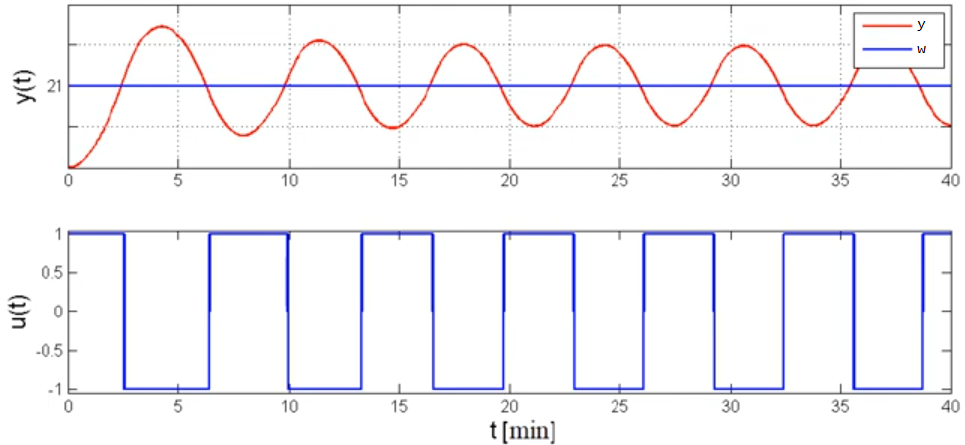
\includegraphics[width=1\linewidth]{25-termostat.png}
    \caption{Wykresy pomiaru, punktu odniesienia oraz wymuszenia w czasie}\label{fig:25-termostat}
\end{figure}

